%%%%%%%% ICML 2019 EXAMPLE LATEX SUBMISSION FILE %%%%%%%%%%%%%%%%%

\documentclass{article}

% Recommended, but optional, packages for figures and better typesetting:
\usepackage{microtype}
\usepackage{graphicx}
\usepackage{subfig}
\usepackage{amsmath}
\usepackage{booktabs} % for professional tables
\usepackage{caption}
\usepackage{tabu}
\usepackage{array}
\usepackage{verbatim}
%\usepackage{natbib}

\graphicspath{ {.} }

% hyperref makes hyperlinks in the resulting PDF.
% If your build breaks (sometimes temporarily if a hyperlink spans a page)
% please comment out the following usepackage line and replace
% \usepackage{icml2019} with \usepackage[nohyperref]{icml2019} above.
\usepackage{hyperref}

% Attempt to make hyperref and algorithmic work together better:
\newcommand{\theHalgorithm}{\arabic{algorithm}}

% Use the following line for the initial blind version submitted for review:
%\usepackage{icml2019}

% If accepted, instead use the following line for the camera-ready submission:
\usepackage[accepted]{icml2019}

% The \icmltitle you define below is probably too long as a header.
% Therefore, a short form for the running title is supplied here:
\icmltitlerunning{Advanced Methods in Natural Language Processing – Spring 2019}
%\setcitestyle{authoryear, open={(},close={)}}

\begin{document}

\twocolumn[
\icmltitle{Convolutional Encoder Approach to Sentence Simplification}

% You can specify symbols, otherwise they are numbered in order.
% Ideally, you should not use this facility. Affiliations will be numbered
% in order of appearance and this is the preferred way.
\icmlsetsymbol{equal}{*}

\begin{icmlauthorlist}
\icmlauthor{Yotam Manne}{equal,tau}
\icmlauthor{Guy Azov}{equal,tau}
\end{icmlauthorlist}

\icmlaffiliation{tau}{Blavatnik School of Computer Science, Tel Aviv University, Tel Aviv, Israel}

\icmlcorrespondingauthor{Yotam Manne}{yotammanne@mail.tau.ac.il}
\icmlcorrespondingauthor{Guy Azov}{guyazov@mail.tau.ac.il}

% You may provide any keywords that you
% find helpful for describing your paper; these are used to populate
% the "keywords" metadata in the PDF but will not be shown in the document
\icmlkeywords{Machine Learning, ICML}

\vskip 0.3in
]


%\printAffiliationsAndNotice{}  % leave blank if no need to mention equal contribution
\printAffiliationsAndNotice{\icmlEqualContribution} % otherwise use the standard text.

\begin{abstract}
Sentence simplification aims to simplify the content and structure of complex sentences, and thus make them easier to interpret for human readers, and easier to process for downstream NLP applications. In this paper, we adapt an architecture of Encoder-Decoder model presented by \cite{DBLP:journals/corr/GehringAGD16}. This model was originally developed for Neural Machine Translation and achieved good results. Due to the similarity of NMT to sentence simplification, we think that this adaption is a natural step in the research of the task.
\end{abstract}

\section{Introduction}
\label{Intro}
The goal of sentence simplification is to convert complex sentences into simpler ones so that they are more understandable and accessible, while still keeping their original information content and meaning. Sentence simplification has a number of practical applications: it is useful for bilingual education and other language-learning contexts. It can help patients with linguistic and cognitive disabilities \cite{Carroll99simplifyingtext}. Sentence simplification can also be used to improve performance in other NLP tasks (\cite{niklaus2017sentence}; \cite{Chandrasekar:1996:MMT:993268.993361};\cite{10.1007/978-3-540-30468-5_47}. Convolutional neural networks (CNN) utilize layers with convolving filters that are applied to
local features. Originally invented for computer vision, CNN models have subsequently been shown to be effective for NLP and have achieved excellent results in semantic parsing \cite{yih2014semantic}, search query retrieval \cite{shen2014learning}, sentence modeling \cite{kalchbrenner2014convolutional}, and other traditional NLP tasks.
In this paper we wish to answer the question whether replacing the classic RNN encoder of a seq2seq model with a convolutional encoder can yield better results in terms of BLEU\cite{papineni2002bleu} and SARI\cite{xu2016optimizing} scores of the output sentences.


\section{Related Work}

In previous studies, researchers of sentence-level simplification mostly address the simplification task as a machine translation problem. \cite{10.1007/978-3-642-12320-7_5} use statistical machine translation approach implemented in Moses toolkit \cite{koehn-etal-2007-moses} to translate the original sentences to the simplified ones. \cite{wang2016text} were the first to suggest using a NMT model for text simplification. They used a LSTM encoder - decoder seq2seq model, but due to the lack of an adequate dataset they used a number-based sequences instead of natural language data. \cite{coster-kauchak-2011-simple} introduced a new dataset of aligned sentence pairs taken from Wikipedia and Simple English Wikipedia, the dataset is widely used in many sentence simplification researches, and set the ground for new and better datasets to be created. \cite{DBLP:journals/corr/ZhangYFZY17} suggested a constrained seq2seq neural model for sentence simplification, their model combines world level and sentence level simplifications and yields better results than various baselines. \citep{meng2015encoding} proposed using a convolutional neural network to encode the source language for NMT. Our work is based on the model that was presented by \cite{DBLP:journals/corr/GehringAGD16} for NMT, which uses two convolutional neural networks as an encoder, and an attention based recurrent neural network as the decoder.

\section{Our Approach}
We chose to adapt a NMT model to the sentence simplification task. Most of the seq2seq neural models we encountered were based on RNN encoder – decoder, however we decided to encode the source sentences with a Convolutional Neural Network instead.
\cite{DBLP:journals/corr/GehringAGD16} used a similar approach for NMT. \cite{di2019enriching} tried it too for sentence classification. But as far as we know, we are the first to try this architecture for sentence simplification.
CNNs computation, contrary to RNNs, can be parallelized, optimization is easier since the number of non-linearities is fixed and independent of the input length and last because they outperform the LSTM accuracy in \cite{DBLP:journals/corr/WuSCLNMKCGMKSJL16}. 

\section{Model (\ref{fig:full})}
\subsection{Encoder Architecture}
One of the challenges of using CNNs encoders is the loss of word ordering. In order to solve it, \cite{DBLP:journals/corr/GehringAGD16} proposes to use position embeddings in addition to the pretrained word embeddings. See table \ref{table:emb}. Let $u_j$ be the $j^{th}$ word in the source sentence, $w_j$ it's word embedding and $l_j$ it's position embedding, then:
\begin{center}
$e_j = l_j + w_j$
\end{center}
%\vspace{5mm}
As suggested by \cite{DBLP:journals/corr/GehringAGD16} The encoder consists of two stacked convolutional networks: CNN-a’s output $z_{j}$ used for creating the attention matrix $A$ that is used at decoding time. Simultaneously, CNN-c’s output $z^{\prime}_{j}$ is used to produce the conditional input $c_i$ by a simple dot product between the attention vector $a_i$ with it.
\vspace{5mm}
\begin{center}
$z_j = CNN_a(\textbf{e})_j,\;z^{\prime}_{j} = CNN_c(\textbf{e})_j$
\vspace{5mm}
\end{center}

The CNNs do not contain pooling layers which are commonly used for down-sampling, i.e., the full source sequence length will be retained after the networks has been applied. \cite{DBLP:journals/corr/GehringAGD16} shows best results when CNN-a contains 2-3 times more layers than CNN-c.


\begin{center}
\begin{table}[h]
 \begin{tabu}  { | X[0.8,l] | X[0.8,l] | X[3,l] | }
 \hline
 Word & Position & Representation \\
 \hline
 we & 1 & WordEmbedding(we) +\linebreak PositionEmbedding(1)  \\ 
 \hline
 need & 2 & WordEmbedding(need) +\linebreak PositionEmbedding(2)\\
 \hline
  a & 3 & WordEmbedding(a) +\linebreak PositionEmbedding(3)\\
 \hline
 vacation & 4 & WordEmbedding(vacation) +\linebreak PositionEmbedding(4)\\
 \hline
\end{tabu}
\caption{Embedding of a full sentence}
\label{table:emb}
\end{table}
\end{center}

\subsection{Decoder Architecture}
\subsubsection{Preliminaries}
\begin{itemize}
\item $h_i$ denotes the hidden state/output of the LSTM.
\item $c_i$ denotes the conditional input to the LSTM.
\item $g_i$ denotes the embedding of the previous output of the LSTM. This gets concatenated with $c_i$ as input to the LSTM
\end{itemize}

\begin{flushleft}

\subsubsection{Attention (\ref{fig:att})}
The attention mechanism is based on the outputs of CNN-c $z^{\prime}_j$. At time step $i$ the conditional input $c_i$ is computed via a dot product attention mechanism \cite{luong2015effective}. We transform the decoder hidden state $h_i$ by a linear layer with weights $W_d$ and $b_d$ to match the size of the embedding of the previous target word $g_i$ and then sum the two representations to yield $d_i$:
\begin{center}
$d_i=W_dh_{i}+b_d+g_i$
\end{center}
Next, we generate the attention matrix $A$ as follows:
$$a_{ij} = \frac{exp \left(d_i^Tz_j\right)}{\sum^m_{t=1}exp\left(d_i^Tz_t\right)}$$
Instead of generating $a_{ij}$ individually, we can generate the entire $\mathbf{a_i}$ in one go, by modifying the equation slightly:
$$\mathbf{a_i} = \text{softmax}(d_i^T\mathbf{z})$$
Finally, we generate $c_i$ as:
$$c_i = \sum_{j=1}^{m}a_{ij}z^{\prime}_{j}$$

\begin{figure}[h]
    \centering
	\captionsetup{justification=centering,margin=2cm}
    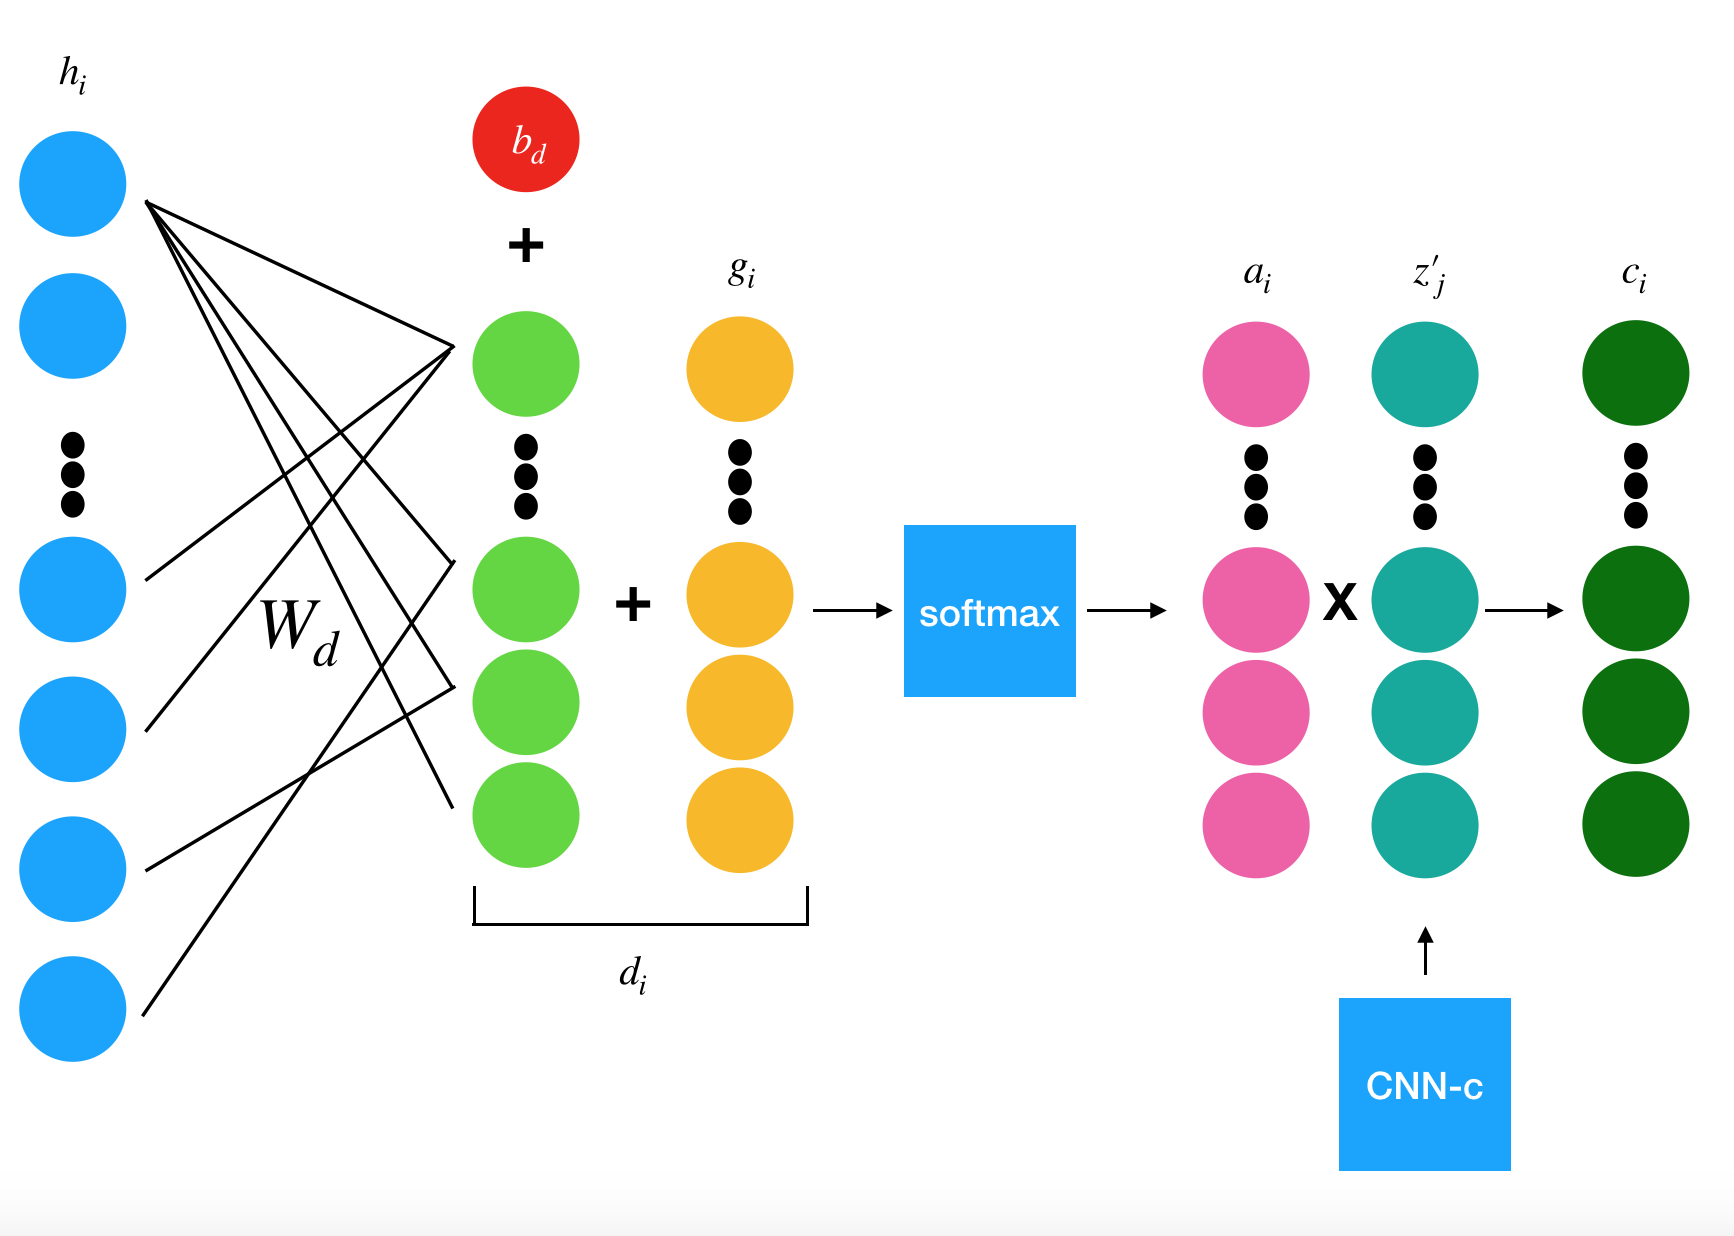
\includegraphics[scale=0.25]{Attention}
    \caption{The dot product attention mechanism}
    \label{fig:att}
\end{figure}

\subsubsection{The Decoder(\ref{fig:dec})}
We use LSTMs \cite{hochreiter1997lstm} for the decoder network whose state $s_i$ comprises of a cell vector and a hidden vector $h_i$ which is output by the LSTM at each time step. We concatenate $c_i$ and $g_i$, and feed them into the LSTM .
The decoder output $h_{i+1}$ is transfromed by a linear layer with weights $W_o$ and bias $b_o$ to the target vocabulary size $V$, then a softmax layer is applied to create a distribution over all possible words. The most probable word will be selected as the decoder's output $y_{i+1}$. 
\vspace{5mm}
\begin{center}
$y_{i+1}=argmax(softmax(W_oh_{i+1}+b_o))$\vspace{5mm}
\end{center}
\end{flushleft}

\begin{figure}[h]
    \centering
	\captionsetup{justification=centering,margin=2cm}
    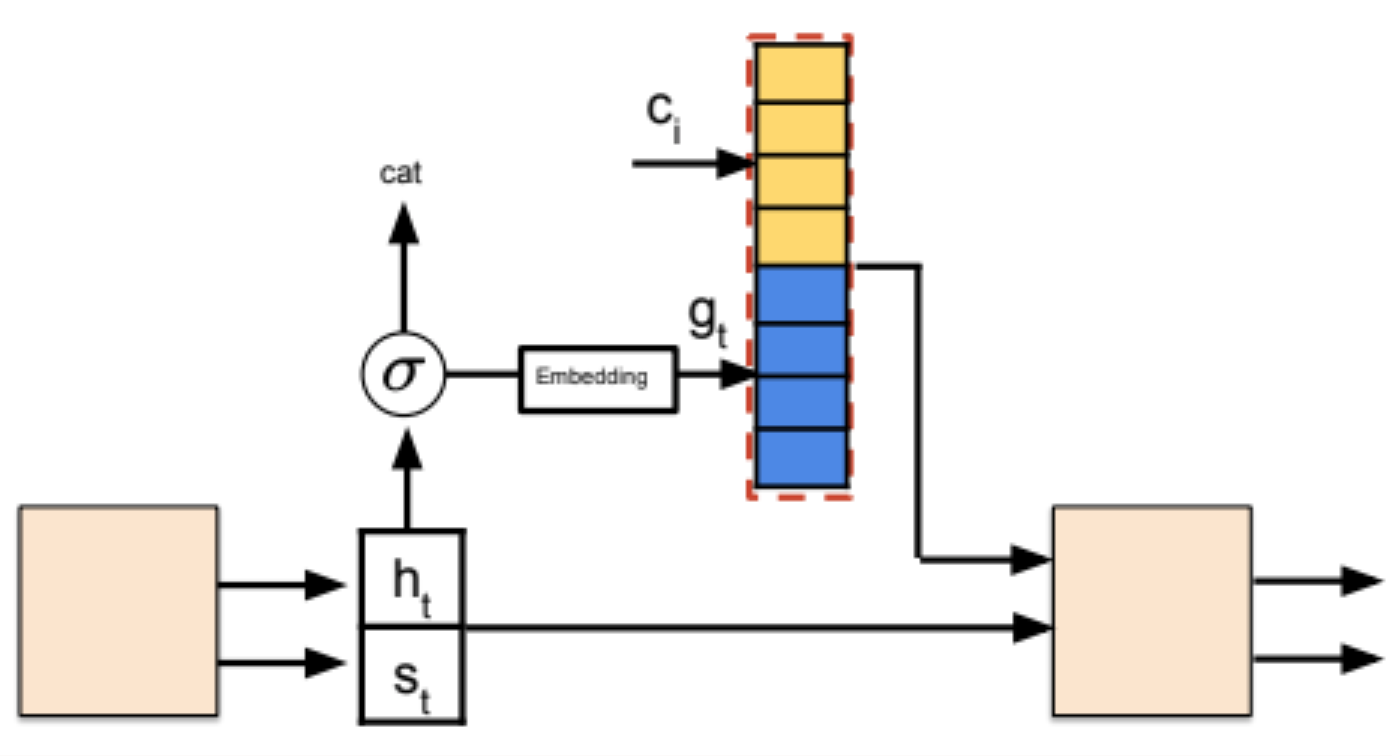
\includegraphics[scale=0.35]{Decoder_Flow}
    \caption{Block diagram of the Decoder flow and architecture}
    \label{fig:dec}
\end{figure}

\begin{figure*}[h]
    \centering
	\captionsetup{justification=centering,margin=2cm}
    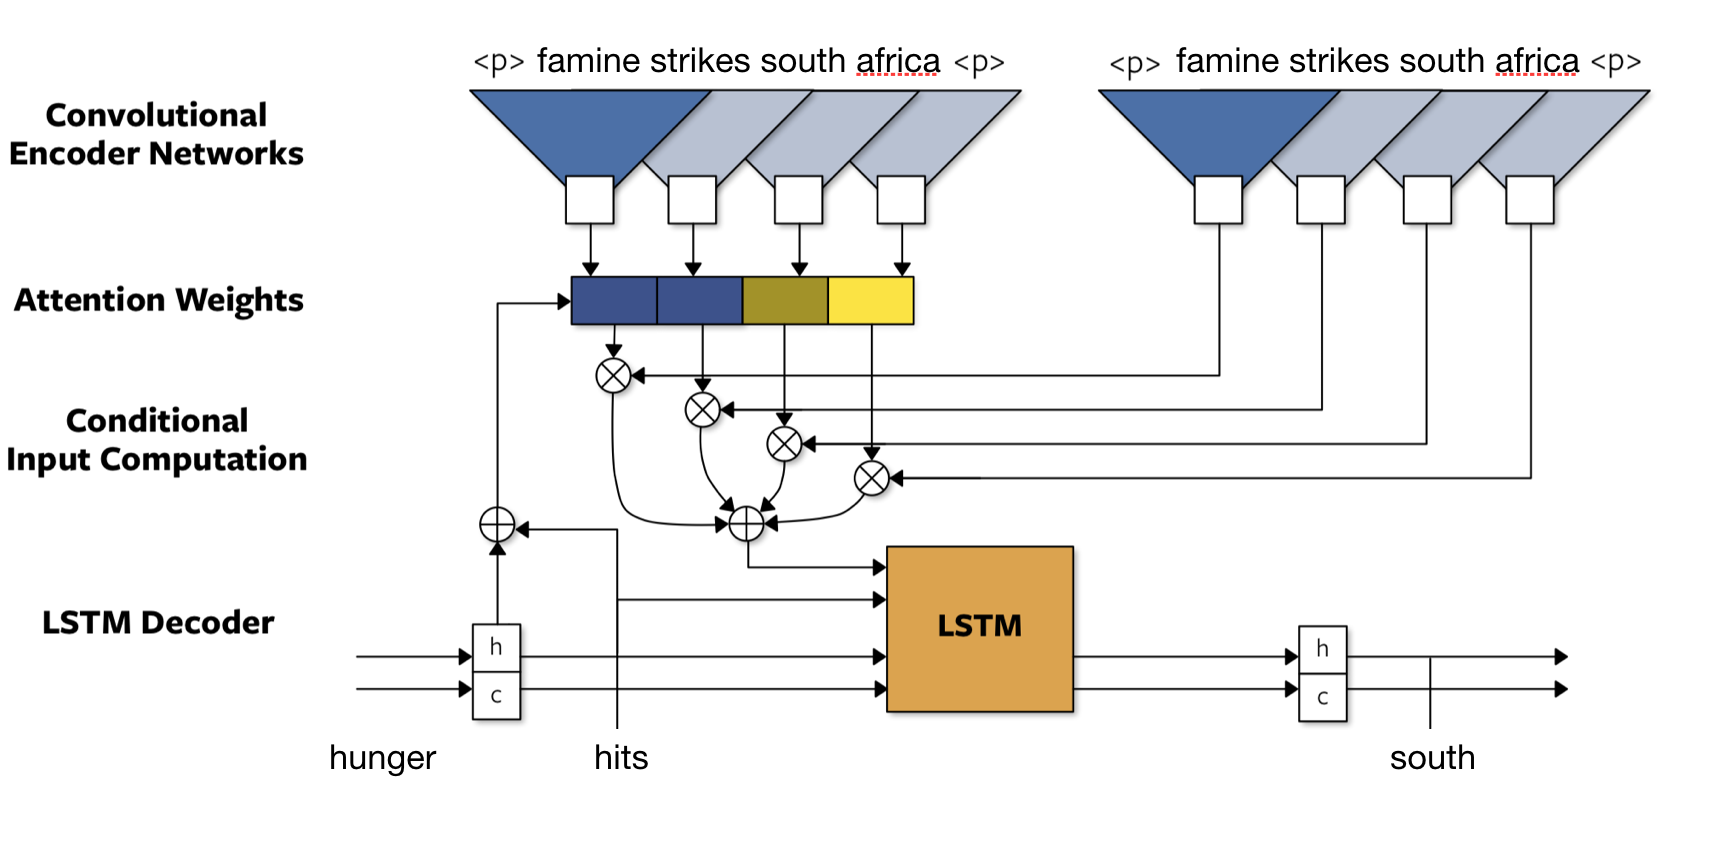
\includegraphics[scale=0.35]{Full_Architecture}
    \caption{Model architecture, adapted from \cite{DBLP:journals/corr/GehringAGD16}}
    \label{fig:full}
\end{figure*}

\section{Experimental Setup}
\subsection{Datasets}
\subsubsection{Simple English Wikipedia \cite{coster-kauchak-2011-simple}}
A sentence aligned dataset taken from parallel articles in English Wikipedia and Simple English Wikipedia. This dataset contains 167K pairs of sentences and is one of the largest datasets used for sentence simplification. While examining this dataset we noticed a few problems – Many sentences contain special characters, URLs, gibberish, excess use of punctuation and more. Such anomalies can corrupt the training procedure and cause unreliable results.

\subsubsection{Newsela \cite{Xu-EtAl:2015:TACL}}
A simplification corpus of news articles, re-written by professional editors to meet the readability standards for children at multiple grade levels. Each sentence in the corpus is rewritten in up to 6 different level of complexity. The creators of this dataset mapped all the problems that exist in the Simple Wikipedia corpus and addressed them in their research. The Newsela dataset contains 141K pairs of aligned sentences.
Our model supports both datasets but because of the problems we mentioned above we used the Newsela corpus for training and evaluation.


\subsection{Data Preprocessing}
To use the data we needed some pre-processing. Two aligned lists of sentences were constructed from the raw data. From each list a vocabulary which maps each word to a unique integer ID was created. Using the mentioned vocabularies, every sentence was converted to a list of word IDs. Each tokenized sentence is fed later as input to our model, which uses GloVe embeddings \cite{pennington2014glove} to represent each word in lower dimensional space.

\subsection{Experiments}
\subsubsection{Control Experiment}
Since we didn’t find any similar models that were tested on the sentence simplification task, we wanted first to get some intuition about the expected results. Therefore we implemented a ‘classic’ LSTM encoder – decoder model and trained it with our dataset. We saw that until the end of the training the loss value was constantly decreasing, which suggests that the model is indeed learning as expected. Nevertheless, when examining the “control model” ’s output over the evaluation set we noticed that the predicted sentences are mostly grammatically correct, but has no contextual relation whatsoever to the input sentence:
\begin{flushleft}
Example:
\begin{itemize}
\item Source: Japanese-American troops were once put in their own units
\item Predicted: Suddenly enemy fighters attacked the patrol
\end{itemize}
\end{flushleft}
While gaining some intuition from the control experiment, it’s results were irrelevant to make any conclusions, so we decided to move on to train and test the main model.


\subsubsection{Main Experiment}
First, for sanity check, we forced the model to overfit over one (small) batch.
Once successful, we tuned the model’s parameters according to \cite{DBLP:journals/corr/GehringAGD16} and \cite{neishi2017bag}. We set the number of layers in CNN-a and CNN-c to 15 and 5 respectively and made residual connection between layers. Each layer consists of 512 hidden units and kernel size of 3. Our decoder consists of a 4 layers bidirectional-LSTM network, with 512 hidden units in each layer.
We used a batch size of 256, and the optimization was done by Adam optimizer \cite{kingma2014adam} with a learning rate of 0.001. To improve learning, we added a Teacher Forcing mechanism \cite{doi:10.1162/neco.1989.1.2.270} with probability 0.5. We limited our scope to sentences up to length 10, in order to focus on the model’s correctness rather than dealing with phenomena related to long sequences. The model was implemented with Pytorch, and training and evaluation were conducted with a single Nvidia Geforce RTX 2080 GPU.

\subsection{Results}
State-of-the-art results in sentence simplification are measured per corpus with two main evaluation metrics:
\begin{itemize}
\item BLEU \cite{papineni2002bleu}
\item SARI \cite{xu2016optimizing}
\end{itemize}
Table \ref{table:results} presents the models that achieved state-of-the-art results to date.
Unfortunately, all our attempts to reach sane results failed badly. All the output sentences consisted of a single word repeating multiple times:
\begin{itemize}
\item Source sentence: "california to help students not fluent in english ."
\item Target sentence: "english language learners get extra help in school"
\item Predicted sentence: "the the the the the the the the the"
\end{itemize}
The loss curve (\ref{fig:loss}) indicated that the model didn't converge. We found it irrelevant to evaluate such results with BLEU or SARI and compare them with state-of-the-art.


\begin{center}
\begin{table}[h]
 \begin{tabu}  { | X[3,l] | X[0.8,l] | X[0.8,l] | }
 \hline
 Model & BLEU & SARI \\
 \hline
 Pointer + Multi-task Entailment and Paraphrase Generation \cite{guo2018dynamic} & 11.14 & 33.22  \\ 
 \hline
 Hybrid \cite{narayan2014hybrid} & 14.46 & 30.00\\
 \hline
  NSELSTM-S (\cite{vu2018sentence} & 22.62 & 29.58\\
 \hline
\end{tabu}
\caption{State-of-the-art sentence simplification results over the Newsela corpus to date.}
\label{table:results}
\end{table}
\end{center}

\begin{figure}[h]
    \centering
	\captionsetup{justification=centering,margin=2cm}
    \includegraphics[scale=0.5]{loss}
    \caption{Loss curve of 1000 epoches of training}
    \label{fig:loss}
\end{figure}

\section{Conclusions and Future Work}
We believe that good results are achievable with our model. We noticed that reaching zero loss in the overfitting test took a great amount of epochs. This might suggest that we were underfitting in the main experiment and that more runtime with stronger hardware can help. \cite{kriz2019complexity} suggested a custom loss function dedicated to sentence simplification that can be integrated and help improve results. We used greedy decoding both in train and evaluation time, however, a beam search algorithm will probably be more accurate. While examining the data we saw that some source sentences differ from their simple version only by 1-2 words. We think that a copy mechanism like the one \cite{mathews2018simplifying} suggested can also increase the model’s accuracy. Due to the lack of convergence of the original model we couldn’t proceed to implementing the improvements above.\linebreak Although it's not a great start in the world of research, the lessons we've learned during this project are priceless. We obtained first intuition of designing and testing a new ML model, and gained valuable experience with Keras and Pytorch libraries. No doubt that in future projects these foundations will help us achieve successful results.

\nocite{*}
\bibliography{example_paper}
\bibliographystyle{icml2019}



\end{document}

